
% !TeX root = ../main.tex
\section{System Architecture}



\begin{figure}[H]
  	\centering   
    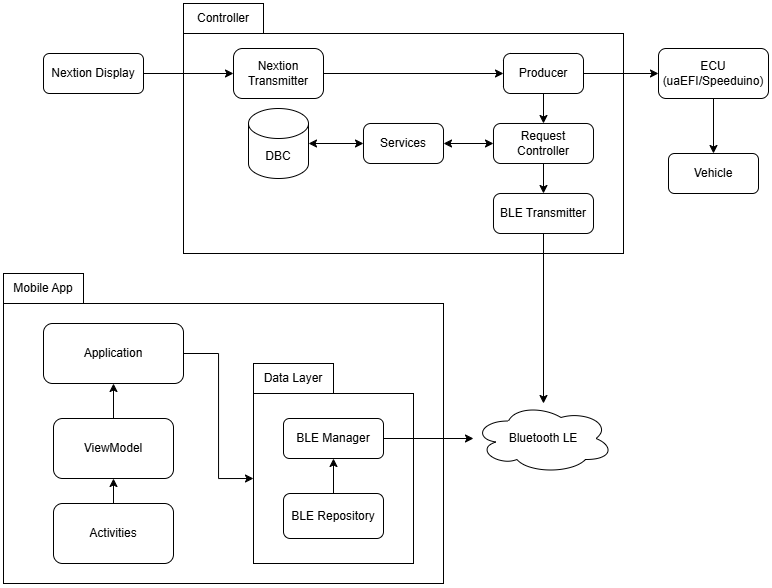
\includegraphics[width=0.8\linewidth]{imagens/project_diagram.png}
    \caption{Project Architecture Diagram}
    \label{fig:prj_arch}
\end{figure}

Figure \ref{fig:prj_arch} illustrates the overall system architecture. The ECU communicates with the Controller via a wired CAN serial link, providing a continuous stream of raw engine frames that are decoded against the vehicle's DBC definition file. At its core sits the Controller, running on the Raspberry Pi Zero 2W, which serves as the central hub for all data acquisition and distribution.  Processed data is simultaneously forwarded to a Nextion display terminal, providing immediate on-site visualisation of critical engine parameters. In parallel, the Controller operates as a Bluetooth Low Energy GATT peripheral, advertising live sensor data to any subscribed central device within range. In the current implementation, an Android mobile application acts as that central, receiving the BLE notifications and presenting the decoded signals in a real-time dashboard. 

\subsection{Controller Configuration File}

The behaviour of the Controller is defined through a JSON configuration file named \texttt{config.json}. This approach separates deployment-specific settings from the application source code, allowing the same software to be adapted to different ECUs, serial interfaces, display devices, and acquisition requirements without modifying its implementation. The file is loaded during application start-up and is also read by the initialization script to determine which hardware interfaces must be available before the Controller is launched.

The \texttt{type} parameter selects the data producer. The value \texttt{rusefi\_can} enables the CAN acquisition path through a GVRET-compatible serial adapter, whereas \texttt{speeduino} \texttt{\_arduino} selects the direct Speeduino serial protocol. The \texttt{mode} parameter selects the local output interface: \texttt{nextion} starts the external Nextion display thread, while \texttt{pi\_screen} starts the PyQt-based interface on a display connected directly to the Raspberry Pi. These parameters allow the acquisition source and the visualization method to be selected independently.

For the \texttt{rusefi\_can} producer, \texttt{com} identifies the serial device associated with the CAN adapter and \texttt{baud\_rate} defines its communication speed. The \texttt{dbc} parameter specifies the path of the DBC file used to translate raw CAN frames into physical vehicle signals. Relative DBC paths are resolved from the Controller directory during start-up. When the \texttt{speeduino\_arduino} producer is selected, the equivalent serial settings are provided through \texttt{port} and \texttt{baudrate}, and \texttt{command} defines the request byte sent to the ECU before each data packet is read. Consequently, only the parameters associated with the selected producer are required during a particular deployment.

Data persistence and diagnostic output are controlled by a separate group of parameters. The \texttt{session\_description} field provides a human-readable description for an acquisition session. The \texttt{state\_save\_interval}, expressed in seconds, determines the minimum interval between consecutive normalized vehicle-state records stored in the database. Raw CAN frames may still be processed at a higher rate, so this value controls database snapshot frequency rather than CAN bus acquisition frequency. The \texttt{log\_can\_activity} flag enables or disables periodic CAN activity messages, while \texttt{can\_log} \texttt{\_interval} determines how frequently the number of received, decoded, and undecoded frames is written to the application log.

The Nextion interface is configured through \texttt{nextion\_port} and \texttt{nextion\_baud}, which define its UART device and communication speed. The \texttt{nextion\_sessions\_interval} parameter determines how frequently the session list is refreshed, and \texttt{nextion\_sessions} \texttt{\_limit} defines the maximum number of sessions presented on the display. The values of \texttt{shift\_point} and \texttt{redline}, both expressed in revolutions per minute, control the RPM visualization: the former determines when the shift indicator changes state, while the latter defines the upper RPM scale used by the dashboard and session graphs.

Finally, \texttt{bluetooth\_enabled} determines whether the BLE server is started together with the Controller. Disabling this option allows acquisition, database storage, and local visualization to continue without exposing the GATT service. The configuration file therefore acts as the central deployment description of the platform, while default values implemented by the software are used for selected optional parameters when they are omitted.

\section{Data Analysis Techniques in Motorsport}
\subsection{Statistical Analysis}

The proposed system records a set of normalized vehicle parameters derived from CAN messages and stored periodically in the database. The currently logged parameters include:

\vspace{-0.2cm}
\begin{table}[H]
\centering
\begin{tabular}{|c|p{12cm}|}
\hline
\textbf{Parameter} & \textbf{Description} \\
\hline

RPM & Engine speed in revolutions per minute, primary indicator of engine operating speed.\\
\hline

SYNC & ECU/engine synchronization status, indicates whether the ECU has valid crankshaft and camshaft position information. \\
\hline

ENGINE & General engine operating status, useful for determining whether the engine is stopped, cranking, or running. \\
\hline

MAP & Intake manifold absolute pressure, one of the primary engine load measurements used for fuel calculations. \\
\hline

BARO & Ambient atmospheric pressure, used for altitude and weather compensation. \\
\hline

TPS & Throttle position, represents driver demand and throttle opening percentage. \\
\hline

IAT & Intake air temperature, affects air density and fueling calculations. \\
\hline

CLT & Engine coolant temperature, critical for warm-up enrichment and engine protection strategies. \\
\hline

AFR & Measured air-to-fuel ratio, key indicator of combustion mixture quality and engine tuning. \\
\hline

EGO & Fuel correction based on oxygen sensor feedback, represents closed-loop fueling adjustments applied by the ECU. \\
\hline

PW & Injector opening duration, directly relates to the amount of fuel delivered to the engine. \\
\hline

VE & Volumetric efficiency used in fuel calculations, represents how effectively the engine fills its cylinders with air. \\
\hline

ADV & Ignition timing advance, major factor of power output, efficiency, and knock resistance. \\
\hline

DWELL & Ignition coil charging time, determines the energy available for spark generation. \\
\hline

BAT & Electrical system voltage, important for injector operation, ignition performance, and system health monitoring. \\
\hline

BOOST & Target boost pressure, desired manifold pressure set by the ECU for forced-induction engines. \\
\hline

DUTY & Wastegate control duty cycle, indicates how aggressively the ECU is controlling boost pressure. \\
\hline

VSS & Vehicle speed, used for logging, speed-based strategies, and traction-related functions. \\
\hline

FAN & Cooling fan status, indicates whether the radiator cooling fan is active. \\
\hline

FP & Fuel pump status, shows whether the ECU has enabled the fuel pump output. \\
\hline

BOOSTCUT & Overboost protection status, indicates whether boost safety limits have been exceeded and protective intervention is active. \\
\hline

\end{tabular}
\caption{ECU Parameters Displayed by the Data Logger}
\label{tab:ecu_parameters}
\end{table}

\section{Hardware development}
\subsection{Hardware schematics}
Our current hardware implementation is comprised of a Raspberry Pi Zero 2W, to which connects a nextion (via serial through the GPIO) and has a USB connection to a GVRET CAN module, which in this case, is a XIAORet, which was also developed in ISEL. \cite{nextion}

The Nextion connection to the raspberry Pi is defined as such:

\begin{figure}[H]
    \centering
    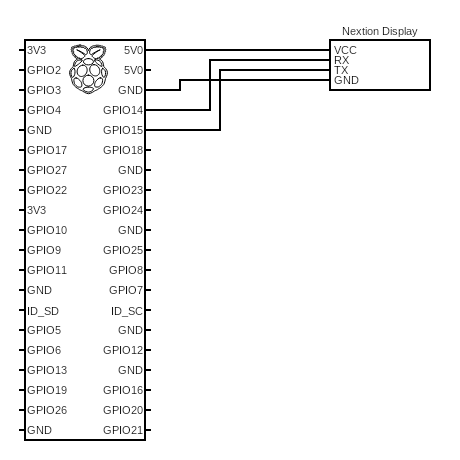
\includegraphics[width=0.5\linewidth]{circuit.png}
    \caption{Electric diagram of the Raspberry Pi and Nextion screen}
    \label{fig:placeholder}
\end{figure}

\subsection{XIAORet comunication protocol}
The XIAORet is a ESP32 microcontroller based CAN Module, that implements the SavvyCan Comunication protocol \cite{savvy}.
SavvyCan is widely used CAN tool for logging, receiving, sending CAN frames and much more. Its widely used in the motorsport world, Formula student and many applications where a CAN tool is needed.
The SavvyCan Comunication protocol is defined as such: 
\begin{itemize}
    \item First, we need enable binary so the following hex command is sent to the XIAORET:0xE7
    \item Secondly, we loop through the received CAN frames, parsing each message. For each frame, the system extracts the timestamp, CAN identifier, data length code (DLC), and payload bytes from the serial stream. The extracted identifier is then processed using a bitmask to ensure compatibility with both standard and extended CAN formats. Subsequently, the frame is matched against the DBC definition, allowing the raw payload to be decoded into meaningful vehicle signals. When a valid mapping is found, the decoded values are integrated into the internal ECU state representation; otherwise, the frame is preserved in its raw form to maintain traceability and support debugging.
\item Although the presented sollution supports 29bit CAN Extended frames, only 11bit CAN Standard frames were tested.
\end{itemize}

\begin{figure}[H]
    \centering
    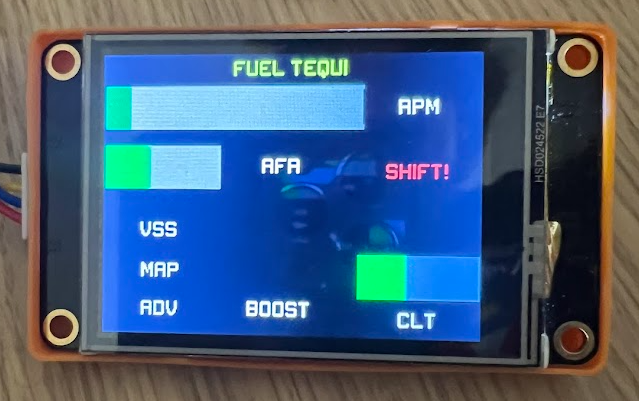
\includegraphics[width=0.5\linewidth]{nextion1.png}
    \caption{Nextion screen 1}
    \label{fig:placeholder}
\end{figure}
\begin{figure}[H]
    \centering
    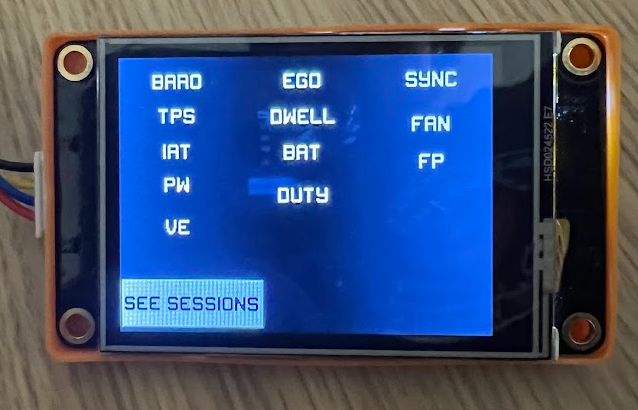
\includegraphics[width=0.5\linewidth]{nextion2.png}
    \caption{Nextion screen 2}
    \label{fig:placeholder}
\end{figure}

\section{Software Implementation}

\subsection{Python Controller}

%\subsubsection{Domain & Repository}

The Python Controller is responsible for several different tasks such as:
\begin{itemize}
    \item \textbf{CAN Connection:} Connection between the ECU module and the Python application using a serial USB link;
    \item \textbf{Database Manager:} Control the database interactions, storing or retrieving the necessary data;
    \item \textbf{UI Display:} Present the information required using a Nextion device, be it real-time from cache or through database requests;
    \item \textbf{Bluetooth Connection and Data Relay:} Connection between the Python application and a connected Bluetooth device (using a mobile app in our implementation).
\end{itemize}

For that end, the application itself has several different inner modules that we will now breakdown and explain, starting with the domain and repository layers.

The \textbf{Domain} and \textbf{Repository} layers are working as a pair since the domain defines the way each data structure is implemented and the repository defines how it gets stored and retrieved. Neither are responsible for the restriction logic - that will be the responsibility of \textit{Services}.

\begin{figure}[H]
    \centering
    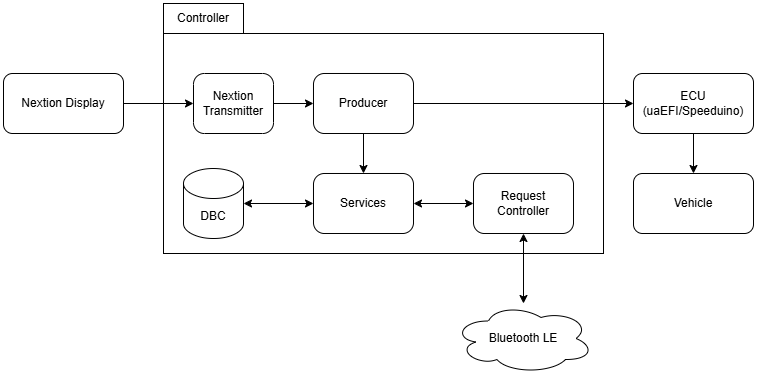
\includegraphics[width=0.8\linewidth]{imagens/controller_diagram.png}
    \caption{Controller Structure Diagram}
    \label{fig:placeholder}
\end{figure}

The domain consists of four different types of classes - \texttt{Session}, \texttt{CANFrame}, \texttt{Signal} and \texttt{VehiculeState} - each used simply to keep information that is either being retrieved or stored in the database.

 A session represents one continuous recording period with a start timestamp, an optional end timestamp that begins as None, and a human-readable description. A \texttt{CANFrame} captures a single raw message off the bus: which session it belongs to, when it arrived, the CAN arbitration ID, the data length code, and the raw data bytes as a string. A Signal is the decoded output of a frame, associating a signal name and its parsed numeric value and unit back to the frame it came from. A \texttt{VehicularState} records the current dataframe state of the vehicle for easy access to the complete information of the vehicle in a specific timestamp. Each domain class has it's respective repository class that will handle the requests to the database.

The repository layer sits directly on top of SQLite database and mirrors that domain structure previously stated. Each repository module opens its own connection to the database at each request and automatically closes said connection when the request is finished using a \texttt{with closing(...)}. This also means that any cross-table operation that needs to be atomic, such as inserting a frame and its signals together, has no transaction boundary protecting it, since each call commits independently. That is an architectural limitation worth addressing before the project handles high-frequency acquisition in production

The services module acts as the single entry point through which the rest of the application interacts with the database. Rather than letting the acquisition pipeline, the UI, or any other consumer reach into a repository directly, everything that needs to read or write persistent data goes through here. In practice every function in the module is a one-liner that receives arguments, forwards them to the appropriate repository function, and returns whatever the repository gives back. The value of this pattern is not in the logic it adds — there is none — but in the boundary it creates: if a repository is ever renamed, replaced, or refactored, only this file needs to change.

We have a class \texttt{SignalCache} that will be the singleton class that will record and transmit the latest dataframe obtain from the ECU and relay it to both the UI Display and the Bluetooth transmission for a faster access to the real-time information.

The BLE transmitter, our bluetooth layer, turns the device into a BLE GATT that an android device is able to discover, connect to and subscribe to continuos sensor data acquired by the ECU. For it's proper operation, we create an instance of \textit{BLETlmServer}, which will build the GATT tree by creating a \texttt{Peripheral} object bound by the device's Bluetooth adapter MAC address and advertising under the local name "\textit{Vehicular\_Monitor}" and will register one primary service and three characteristics under that service. The first characteristic will be configured with both \texttt{read} and \texttt{notify} flags in order for the mobile client to either poll the data explicitly or to be notified of any updates to the signal cache. This way we can attach two different callback: \texttt{read\_callback} and \texttt{notify\_callback}. The second characteristic will be configured with \texttt{write} flag in order to obtain session requests from the mobile client and has a \texttt{\_session\_request\_cb} as a \texttt{write\_callback}. This characteristic exists to be able to accurately send requested information through the third characteristic. The third characteristic is similar to the first one with different callbacks: \texttt{\_session\_response\_read\_cb} and \texttt{\_session\_response\_notify\_cb}

The notify mechanism is the most important part to understand correctly. In \textit{Bluezero}, \texttt{notify-callback} is not a function that gets called each time a notification needs to be sent — it is a status callback that fires once when a client subscribes and once when it unsubscribes. When it fires with \texttt{notifying=True}, the callback receives a reference to the live characteristic object and immediately schedules a repeating GLib timer set to fire every 200 milliseconds. Each time the timer fires, \texttt{\_send\_notify} calls \texttt{characteristic.set\_value()} with the latest encoded cache string, which emits a D-Bus \texttt{PropertiesChanged} signal that BlueZ translates into an actual BLE notification packet sent to the Android device. The timer returns True on every successful call to keep itself alive, and only returns False — which removes it — if the characteristic reference has been cleared. When the client unsubscribes and notify\_cb fires with notifying=False, the stored characteristic reference is cleared and the GLib timer is cancelled with GLib.source\_remove, stopping all further transmissions until a new subscription arrives.

As mentioned before, the BLE transmitter utilizes two characteristics in charge of obtaining session requests and returning session responses towards the remote device. These characteristics allow the use of several different commands: the session list (format: \texttt{"GET\_SESSIONS"}), session information by identifier (format: \texttt{"GET\_SESSION:\_ID\_"} ), session creation (format: \texttt{"CREATE\_SESSION"}), and session ender (format: \texttt{"END\_SESSION"}). These commands either return a list of values obtained from the database, or a boolean in case of error, and are available to any application that is connected to the available service provided by the python controller and is connected through BLE. 

Calling start() triggers ble.publish(), which begins advertising the peripheral and hands control to the GLib main loop. This call never returns under normal operation — everything that needs to happen alongside the BLE server, such as the mock data generator or the console status printer, must be running in daemon threads before start() is called. The process must also be launched with \textit{sudo ./venv/bin/python3} rather than bare sudo python3, because BlueZ requires root privileges and the system Python does not have bluezero installed.

\subsection{Python Producer}

The Python producer application constitutes the core of the proposed CAN platform controller, being responsible for data acquisition, processing, storage, and visualization. The system is implemented in Python and follows a modular, multi-threaded architecture designed to ensure high performance, scalability, and maintainability. Both the controller are integrated and running in the same processor as a way to not only obtain all necessary information through the producer and implement all required functionality through the controller.

From an architectural perspective, the application adopts a distributed processing model based on multiple worker threads. This approach allows different responsibilities such as data acquisition, decoding, persistence, and visualization to be executed concurrently. As a result, the system minimizes bottlenecks and ensures real-time responsiveness when handling high-frequency CAN data streams.

The application entry point is defined in \textit{main.py}, which orchestrates the system initialization workflow. At startup, the application reads a configuration file (\textit{config.json}) that defines both the data source (\textit{producer type}) and the output interface (\textit{mode}). This configuration-driven design enables flexibility, allowing the same software to operate with different ECUs and visualization methods without requiring code modifications.

Following configuration loading, the system initializes the SQLite database (\textit{ecu\_data.db}) and ensures that all required tables are created. These include tables for raw CAN frames, acquisition sessions, and normalized vehicle state snapshots. The database layer is abstracted through a repository pattern, which decouples data persistence from the rest of the application logic and improves maintainability.


\begin{figure}[H]
    \centering
    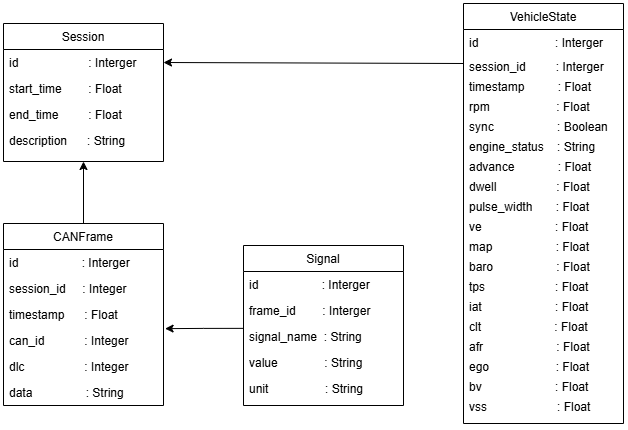
\includegraphics[width=0.7\linewidth]{imagens/db_diagram.png}
    \caption{Database Diagram}
    \label{fig:placeholder}
\end{figure}

The data acquisition process is handled by a dedicated producer thread, which can operate in different modes depending on the selected ECU interface. In the \textit{rusefi\_can} mode, the system reads CAN frames via a SavvyCan-compatible serial adapter. These frames are decoded using a DBC file, allowing raw binary messages to be translated into meaningful automotive signals. Alternatively, in the \textit{speeduino\_arduino} mode, the application directly parses structured serial data packets via USB, from the Speeduino ECU.

Decoded signals are then mapped into a unified internal representation of the vehicle state. This state is maintained in a shared memory structure called \textit{signal\_cache}, which always stores the most recent values received from the ECU. This design avoids repeated database queries and enables fast access for visualization components.

In parallel with the acquisition process, additional threads handle data persistence and output. The system periodically stores snapshots of the vehicle state in the database, enabling offline analysis while retaining the raw CAN traffic required for traceability.

\subsubsection{CAN Data Persistence and Session Recording}

Database recording is organized around acquisition sessions. The Controller continues to acquire and decode CAN traffic immediately after start-up, but persistent recording only begins when a session has been created. In the present Nextion workflow, the display starts a session by transmitting a \texttt{NEW\_SESSION} request. If another session is already active, its end timestamp is recorded before a new row is inserted into the \texttt{sessions} table. Each subsequent database record is associated with the identifier of the active session. Before this request is received, decoded data remains available to the live display and Bluetooth interface through the signal cache, but it is not written to the session tables.

Two complementary forms of data are stored during a session. First, every valid GVRET CAN frame is inserted into the \texttt{can\_frames} table, including frames whose identifiers are absent from the DBC file or whose payload cannot be mapped to the normalized vehicle state. Each row contains the session identifier, reception timestamp, CAN identifier, data length code, and hexadecimal payload. This provides a complete record of the received bus traffic and preserves undecoded frames for subsequent inspection or reprocessing. The current implementation performs and commits each insertion individually rather than grouping several frames into a transaction.

Second, decoded frames update an in-memory aggregate containing the latest known value of every supported vehicle parameter. Since the RusEFI base messages distribute related signals across several CAN identifiers, an individual decoded frame generally modifies only part of this aggregate. For example, one message updates engine speed, ignition advance, and vehicle speed, while another updates manifold pressure and temperatures. Values obtained from earlier messages are retained until they are replaced, allowing the aggregate to represent the most recent complete vehicle state.

A copy of this aggregate is periodically inserted into the \texttt{vehicle\_state} table. The minimum interval between consecutive snapshots is defined by the \texttt{state\_save\_interval} configuration parameter, expressed in seconds. With a value of \texttt{1.0}, the system records approximately one vehicle-state row per second; values of \texttt{0.5} and \texttt{0.25} allow maximum rates of approximately 2 and 4~Hz, respectively. The interval is evaluated when a decoded frame arrives, rather than by an independent timer. Consequently, a snapshot is written on the first decoded frame received after the configured interval has elapsed. No state is stored during periods in which no decodable traffic is received, and the actual spacing may therefore be slightly greater than the configured value.

The snapshot interval is reset whenever the active session changes, causing the first decoded frame of a new session to be recorded immediately. Each \texttt{vehicle\_state} row contains the session identifier, insertion timestamp, and the complete normalized set of engine, load, temperature, fuelling, ignition, electrical, boost, speed, and status parameters. Its timestamp is generated by the Raspberry Pi at insertion time. By contrast, raw CAN frame rows use the frame reception time captured by the acquisition process. The adapter-provided GVRET timestamp is used during parsing but is not presently persisted as a separate database field.

This separation provides different resolutions for different purposes. The \texttt{can\_frames} table follows the incoming bus rate and maintains the detailed source record, whereas \texttt{vehicle\_state} contains a lower-frequency time series suitable for session graphs and general analysis. For example, a ten-minute session with a snapshot interval of one second produces approximately 600 vehicle-state rows, while the number of raw frame rows depends directly on CAN traffic and may be several orders of magnitude higher. Session graph requests query \texttt{vehicle\_state}, filter rows by session identifier, and order them by timestamp before the selected parameters are plotted.

The database schema also contains a \texttt{signals} table intended to associate individually decoded values with their source CAN frames. This table is supported by the repository layer but is not populated by the current GVRET acquisition path; normalized values are instead retained through the periodic \texttt{vehicle\_state} snapshots. Furthermore, equivalent persistence has not yet been integrated into the \texttt{speeduino\_arduino} reader, which currently updates the live signal cache without creating raw-frame or vehicle-state records. These constraints define the present recording scope and identify areas for future development, particularly transaction batching, explicit session termination during shutdown, and a common persistence path for both supported producers.

For visualization, the application supports two independent output modes. In the \textit{Nextion} mode, a dedicated thread continuously reads the latest values from the \textit{signal\_cache} and transmits them over a serial interface to a Nextion display, providing a lightweight, embedded graphical interface. In the \textit{pi\_screen} mode, a PyQt-based dashboard runs locally on the Raspberry Pi, periodically refreshing the displayed values using a timer mechanism. The separation between data acquisition and visualization ensures that user interface performance does not interfere with real-time data processing.

\subsubsection{Nextion Session Graph Generation}

In addition to displaying live values, the Nextion interface can plot signals stored during a previous acquisition session. A graph request issued by the display identifies the selected session and the signals to be represented. The Controller resolves the displayed session index to its database identifier, retrieves the corresponding vehicle-state records, and converts the resulting series into native Nextion drawing commands. The graph is therefore rendered by the display itself using line, fill, and text commands, without transferring a bitmap or relying on the Nextion waveform component.

The plotting area begins at coordinate $(35,45)$ and has a width of 410 pixels and a height of 170 pixels. Samples are distributed uniformly along the horizontal axis, from $x=35$ to $x=445$, according to their order in the retrieved series. For a series containing $N$ samples, the horizontal coordinate of sample $i$ is given by

\begin{equation}
x_i = 35 + \left\lfloor \frac{i}{N-1} \times 410 \right\rfloor .
\end{equation}

This representation assumes that stored vehicle-state samples are separated by approximately regular intervals. When a session contains more than 410 records, the series is reduced to 410 uniformly selected samples. Both endpoints are retained, ensuring that the complete session is represented while limiting the number of serial commands and avoiding multiple samples being assigned to the same horizontal pixel.

Each signal is normalized independently on the vertical axis using a predefined physical range. If $v_i$ is the measured value, and $v_{\min}$ and $v_{\max}$ are the limits assigned to that signal, its vertical coordinate is calculated as

\begin{equation}
y_i = 45 + 170 - \left\lfloor
\frac{v_i-v_{\min}}{v_{\max}-v_{\min}} \times 170
\right\rfloor .
\end{equation}

Values outside the specified range are clamped to the upper or lower graph boundary. The inversion in this expression is required because the Nextion coordinate system places the origin at the top-left corner of the screen. Consequently, a signal's minimum value is plotted at $y=215$, its midpoint at approximately $y=130$, and its maximum at $y=45$.

The ranges used by the implementation are listed in Table~\ref{tab:nextion_graph_ranges}. The RPM upper limit is obtained from the configurable \texttt{redline} value; the remaining limits are fixed according to the expected operating range of each parameter.

\begin{table}[H]
\centering
\begin{tabular}{|l|c|c|l|}
\hline
\textbf{Signal} & \textbf{Minimum} & \textbf{Maximum} & \textbf{Unit} \\
\hline
Engine speed (RPM) & 0 & \texttt{redline} & rpm \\
Air--fuel ratio (AFR) & 10 & 20 & -- \\
Coolant temperature (CLT) & 0 & 120 & $^{\circ}$C \\
Intake air temperature (IAT) & 0 & 80 & $^{\circ}$C \\
Throttle position (TPS) & 0 & 100 & \% \\
Manifold pressure (MAP) & 0 & 250 & kPa \\
Barometric pressure (BARO) & 80 & 120 & kPa \\
Ignition advance (ADV) & $-20$ & 60 & degree \\
Injector pulse width (PW) & 0 & 20 & ms \\
Battery voltage (BAT) & 0 & 16 & V \\
Boost target & 0 & 250 & kPa \\
Boost duty & 0 & 100 & \% \\
Vehicle speed (VSS) & 0 & 250 & km/h \\
\hline
\end{tabular}
\caption{Vertical scales used for Nextion session graphs}
\label{tab:nextion_graph_ranges}
\end{table}

After coordinate conversion, consecutive points belonging to the same signal are joined by line commands. Up to six signals can be distinguished using the predefined red, blue, green, orange, cyan, and magenta sequence; colours are reused if additional signals are requested. Since every signal uses its own vertical scale, overlapping curves indicate a similar relative position within their respective operating ranges rather than equality of their physical values. This normalization allows parameters with different units and magnitudes, such as RPM, AFR, and coolant temperature, to be inspected together within the limited display area.

To support deployment as an embedded system, the application includes an initialization script (\textit{init.sh}) designed to be executed as a systemd service (or first time startup). This script prepares the runtime environment, waits for required hardware interfaces (such as serial devices), and guarantees automatic startup and recovery in case of failure. This makes the system robust and suitable for unattended operation in automotive environments.

Overall, the combination of a multi-threaded architecture, modular design, configuration-driven behavior, and efficient data handling mechanisms allows the Raspberry Pi application to meet the real-time requirements of vehicular data acquisition systems while maintaining flexibility and extensibility for future developments.

\clearpage
\subsection{Android application}

The Android application is utilized as an exterior module to the Python Controller that will receive data via BLE from the controller and display it in an intuitive manner. This module could be replaced for any other application as long as it follows the communication protocol defined by the controller and be connected to the controller via Bluetooth.

\begin{figure}[H]
    \centering
    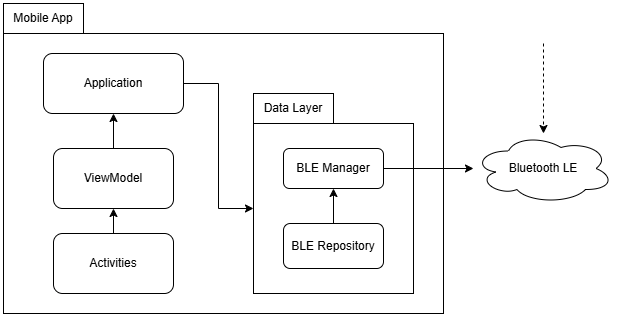
\includegraphics[width=0.8\linewidth]{imagens/mobile_diagram.png}
    \caption{Mobile Application Structure Diagram}
    \label{fig:placeholder}
\end{figure}

The structure of the Android application is as follows:
\begin{itemize}
    \item \textbf{Application:} Root of the entire dependency structure and implements the \texttt{Dependency Container} interface that declares three different singletons - \texttt{Ble Manager}, \texttt{Ble Repository} and \texttt{BleViewModelFactory} - available to the rest of the application
    \item  \textbf{Activity:} All activities extend \texttt{BaseActivity} and are the boundary between the application and it's UI. \texttt{BaseActivity} standardizes lifecycle logging across every screen and exposes a generic \texttt{navigate<T>()} helper used to move between activities, as well as a {backPressed()/backAware()} hook for consistent back-navigation handling. The \texttt{MenuActivity} is the primary activity. It manages the application permissions (\texttt{BLUETOOTH\_SCAN} and \texttt{BLUETOOTH\_CONNECT} and \texttt{ACCESS\_FINE\_LOCATION}) and starts the scanning for connected Bluetooth devices, working as a link to distribute said Bluetooth device's information to the rest of the possible activities. Selecting a scanned device opens \texttt{DeviceMenuActivity}, a per-device menu (Live Data, Sessions Information, Overall Statistics, Device Information) that in turn opens \texttt{DataDisplayActivity} to show the live data stream for that device. \texttt{AboutActivity} is reachable from \texttt{MenuActivity} and shows application information.
    \item \textbf{ViewModel:} The core of the application's state management through \texttt{BleViewModel}. It holds the current state \texttt{\_uiState} of the current application and exposes it in a immutable \textit{StateFlow} to the current observable screen. When \texttt{.start()} is called, it launches a coroutine that collects cvs strings from \texttt{BleRepository.canData} and when \texttt{.connect()} is called it passes the selected device to the repository to initiate GATT connection. Each incoming csv line is parsed by \texttt{parseCanData()} into a \texttt{MainUiState} carrying the individual channels reported by the controller (RPM, coolant temperature, AFR, TPS, MAP, battery voltage, dwell, ignition timing, VSS, IAT, EGO correction, VE, and sync status), with the raw string preserved alongside the parsed fields. For development and demonstration without a physical controller connected, \texttt{BleViewModel} also exposes \texttt{.startMockData()}, which generates a continuous stream of plausible randomized values into the same uiState so the UI can be exercised standalone. \texttt{BleViewModelFactory} allows the construction of a \texttt{BleViewModel} with the \texttt{BleRepository} constructor.
    \item \textbf{Model:} The \texttt{BleManager} owns every interaction with the Android Bluetooth stack, scanning for devices, loading already-paired (bonded) devices, and connecting over GATT using a service and three different characteristics that forms part of the defined communication protocol with the controller. \texttt{BleRepository} wraps \texttt{BleManager} as a stable boundary. It re-exposes \texttt{devicesFlow} and \texttt{dataFlow} as \texttt{scannedDevices} and \texttt{canData} respectively, and delegates \texttt{startScan} and \texttt{connectToDevice} directly. Its presence means the \texttt{ViewModel} layer imports nothing from \texttt{BleManager} directly, and the BLE implementation could be replaced or mocked entirely without touching a single \texttt{ViewModel}.
\end{itemize}
